

\def\qtr{Spring 2023}
\def\due{Wednesday, May 24 at 11:59 pm}
\def\edstem{\url{https://edstem.org/us/courses/37893/discussion/}}
\def\psetnum{3 }

%%% Change the following flag to toggle between questions or solutions
\ifdefined\solutions {} \else \def\solutions{1} \fi


\documentclass{article}

\usepackage{graphicx}

\newcommand{\di}{{d}}
\newcommand{\nexp}{{n}}
\newcommand{\nf}{{p}}
\newcommand{\vcd}{{\textbf{D}}}

\usepackage{nccmath}
\usepackage{mathtools}
\usepackage{graphicx,caption}
\usepackage{enumitem}
\usepackage{epstopdf,subcaption}
\usepackage{psfrag}
\usepackage{amsmath,amssymb,epsf}
\usepackage{verbatim}
\usepackage{url}
\usepackage[hang,flushmargin]{footmisc} 
\usepackage{hyperref}
\newcommand{\hurl}[1]{\href{#1}{#1}}
\renewcommand{\url}{\nolinkurl}
\AtBeginDocument{
	\label{CorrectFirstPageLabel}
	\def\fpage{\pageref{CorrectFirstPageLabel}}
}
\usepackage{color}
\usepackage{bbm}
\usepackage{listings}
\usepackage{setspace}
\usepackage{float}
\usepackage{natbib}
\definecolor{Code}{rgb}{0,0,0}
\definecolor{Decorators}{rgb}{0.5,0.5,0.5}
\definecolor{Numbers}{rgb}{0.5,0,0}
\definecolor{MatchingBrackets}{rgb}{0.25,0.5,0.5}
\definecolor{Keywords}{rgb}{0,0,1}
\definecolor{self}{rgb}{0,0,0}
\definecolor{Strings}{rgb}{0,0.63,0}
\definecolor{Comments}{rgb}{0,0.63,1}
\definecolor{Backquotes}{rgb}{0,0,0}
\definecolor{Classname}{rgb}{0,0,0}
\definecolor{FunctionName}{rgb}{0,0,0}
\definecolor{Operators}{rgb}{0,0,0}
\definecolor{Background}{rgb}{0.98,0.98,0.98}
\lstdefinelanguage{Python}{
numbers=left,
numberstyle=\footnotesize,
numbersep=1em,
xleftmargin=1em,
framextopmargin=2em,
framexbottommargin=2em,
showspaces=false,
showtabs=false,
showstringspaces=false,
frame=l,
tabsize=4,
% Basic
basicstyle=\ttfamily\footnotesize\setstretch{1},
backgroundcolor=\color{Background},
% Comments
commentstyle=\color{Comments}\slshape,
% Strings
stringstyle=\color{Strings},
morecomment=[s][\color{Strings}]{"""}{"""},
morecomment=[s][\color{Strings}]{'''}{'''},
% keywords
morekeywords={import,from,class,def,for,while,if,is,in,elif,else,not,and,or
,print,break,continue,return,True,False,None,access,as,,del,except,exec
,finally,global,import,lambda,pass,print,raise,try,assert},
keywordstyle={\color{Keywords}\bfseries},
% additional keywords
morekeywords={[2]@invariant},
keywordstyle={[2]\color{Decorators}\slshape},
emph={self},
emphstyle={\color{self}\slshape},
%
}


\pagestyle{empty} \addtolength{\textwidth}{1.0in}
\addtolength{\textheight}{0.5in}
\addtolength{\oddsidemargin}{-0.5in}
\addtolength{\evensidemargin}{-0.5in}
\newcommand{\ruleskip}{\bigskip\hrule\bigskip}
\newcommand{\nodify}[1]{{\sc #1}}
\newcommand{\points}[1]{{\textbf{[#1 points]}}}
\newcommand{\subquestionpoints}[1]{{[#1 points]}}
\newenvironment{answer}{{\bf Answer:} \sf \begingroup\color{red}}{\endgroup}%

\newcommand{\bitem}{\begin{list}{$\bullet$}%
{\setlength{\itemsep}{0pt}\setlength{\topsep}{0pt}%
\setlength{\rightmargin}{0pt}}}
\newcommand{\eitem}{\end{list}}

\setlength{\parindent}{0pt} \setlength{\parskip}{0.5ex}
\setlength{\unitlength}{1cm}

\renewcommand{\Re}{{\mathbb R}}
\newcommand{\R}{\mathbb{R}}
\newcommand{\what}[1]{\widehat{#1}}

\renewcommand{\comment}[1]{}
\newcommand{\mc}[1]{\mathcal{#1}}
\newcommand{\half}{\frac{1}{2}}

\def\KL{D_{KL}}
\def\xsi{x^{(i)}}
\def\ysi{y^{(i)}}
\def\zsi{z^{(i)}}
\def\E{\mathbb{E}}
\def\calN{\mathcal{N}}
\def\calD{\mathcal{D}}

\newcommand{\diag}{\mathop{\rm diag}}
\newcommand{\logisticloss}{\ell_{\textup{logistic}}}
\newcommand{\softmax}{\textup{softmax}}
\usepackage{tikz}
\usepackage{bbding}
\usepackage{pifont}
\usepackage{wasysym}
\usepackage{amssymb,amsthm}
\usepackage{booktabs}
\usepackage{verbatim}


\newtheorem{lemma}{Lemma}

\def\shownotes{0}  %set 1 to show author notes
\ifnum\shownotes=1
\newcommand{\authnote}[2]{[#1: #2]}
\else
\newcommand{\authnote}[2]{}
\fi

\newcommand{\tnote}[1]{{\color{blue}\authnote{TM}{#1}}}
\newcommand{\fk}[1]{{\color{purple}{[FK:#1]}}}
\newcommand{\notes}[1]{{\color{blue} Note:} \textit{#1} \newline}



\usepackage{dsfont}

\begin{document}

\pagestyle{myheadings} \markboth{}{CS229 Problem Set \#\psetnum}

\ifnum\solutions=1{
{\huge\noindent CS 229, \qtr\\
Problem Set \#\psetnum Solutions}\\\\
YOUR NAME HERE (\texttt{YOUR SUNET HERE})
} \else {\huge
\noindent CS 229, \qtr\\
Problem Set \#\psetnum
} \fi

\ruleskip

{\bf Due {\due } on Gradescope.}

\medskip

\item \points{35} {\bf Reinforcement Learning: Policy Gradient}

Before working on this problem, please run \texttt{pip install gym==0.17.3} to install the OpenAI Gym Python dependency.

In this problem you will investigate reinforcement learning, in particular policy gradient methods, as an approach to solving control tasks without explicit knowledge of the dynamics of the underlying system.

The problem we will consider is the inverted pendulum problem, also referred to as the pole-balancing problem, provided in the form of the {\tt CartPole-v0} OpenAI Gym environment.\footnote{{\tt https://gym.openai.com/envs/CartPole-v0/}} 
The physics setup and details of the MDP are described below, although you do not necessarily have to understand all the details to solve the problem. 
As shown in the figure below, a thin pole is connected via a free hinge to a cart, which can move laterally on a smooth table surface. 
Our objective is to develop a controller/policy to balance the pole with these  constraints by appropriately having the cart accelerate either left or right. The controller/policy is considered as failed if either the angle of the pole deviates by more than a certain amount from the vertical position (i.e., if the pole falls over), or if the cart's position goes out of bounds (i.e., if it falls off the end of the table by going too far left or right). 

\begin{center}
  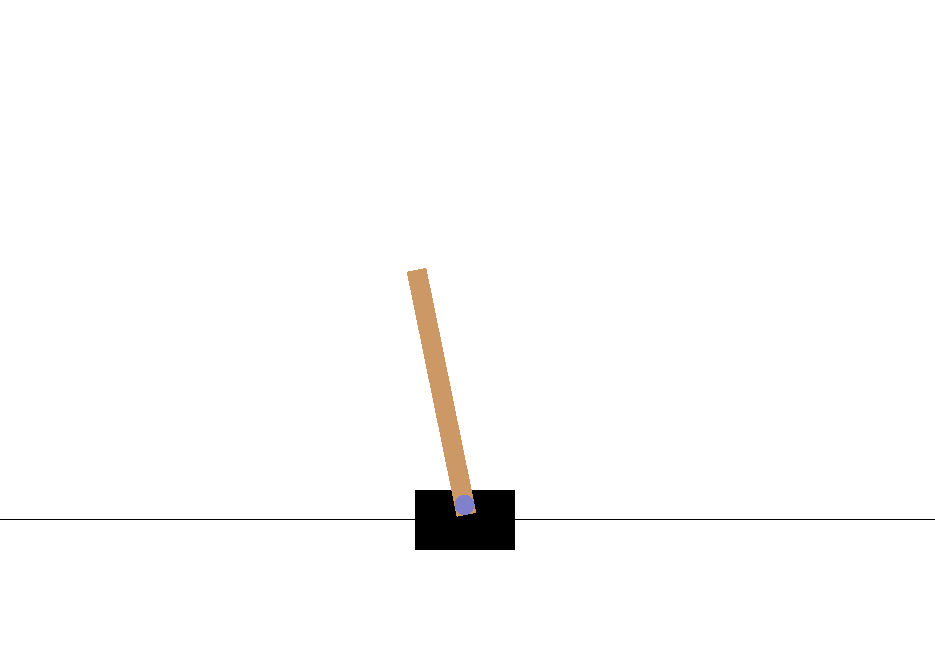
\includegraphics[width=8cm]{policy_gradient/env.png}
\end{center}

We have included a simple simulator for this problem. The simulation proceeds in discrete time cycles (steps). The state of the cart and pole at any time is completely characterized by 4 scalar values: the cart position, the cart velocity, the angle of the pole measured as its deviation from the vertical position, and the angular velocity of the pole. The concatenation of these 4 scalar values is the state $s$. 

\newcommand{\tilT}{\tilde{T}}
At every time step, the controller must choose one of two actions: push (accelerate) the cart left, or push the cart right. (To keep the problem simple, there is no {\it do-nothing} action.) \textbf{These are represented as actions $0$ and $1$ respectively in the code.}  When the action choice is made, the simulator updates the state according to the underlying dynamics, and provides a new state. 
If the angle of the pole deviates by more than a certain amount from the vertical position, or if the cart's position goes out of bounds, we conceptually consider that the MDP enters a special ``done'' state, and once the MDP enters the ``done'' state, no actions can recover it to any normal state. 
We choose the horizon $T$ to be 200, meaning, we only take at most 200 actions in each trajectory. Note because once the system enters the ``done'' state, it stays there forever, we do not have to simulate the MDP and sample more states anymore after the first time we enter the done state (and all future done states can be ignored because no actions can influence anything). Therefore, in the code, you will only interact with the simulation until the system hits the done state (or reaches a trajectory length of 200), so the effective length of the trajectory can be less than 200. We use $\tilT$ to denote the number of steps with which a trajectory reaches a ``done'' state or 200 otherwise. The discount factor will be set to $\gamma=1$ throughout the question. 


Our goal is to make the pole and cart stay in bounds without entering the done state for as many steps as possible. To do this, we design the following reward function.  For any normal state $s\in \R^4$, we have $R(s)=1$ (and $R$ does not depend on the action $a$). When the system is at the ``done" state (that is, the pole angle goes beyond a certain limit or when the cart goes too far out), the reward is 0. The reward is given to you in the code as part of the MDP. 

The files for this problem are contained within the \texttt{src/policy\_gradient/} directory. Most of the scaffolding code has already been written for you, and you need to make changes only to {\tt policy\_gradient.py} in the places specified. There are also several details that are also clearly outlined inside of the code. This file can then be run to display the behavior of the agent in real time, and to plot a learning curve of the agent at the end.

\begin{enumerate}
\item \subquestionpoints{6} 
\textbf{Policy Gradient}

In this part, we will fully detail the characterization of our policy gradient method and derive the update rule to train our model to solve the {\tt CartPole-v0} environment.

In this problem we will be learning a \textit{logistic} policy. This means that our policy will be a sigmoid function of a linear function in the state. 
Recall that the sigmoid function $\sigma(z) = 1 / (1 + e^{-z})$. Let $\theta \in \R^4$ be the parameters of the policy. 
The probability of taking action 0 (left) is parameterized by 
\begin{align*}
    \pi_\theta(0 | s) &= \sigma(\theta^\top s) 
\end{align*}
Given that our environment only contains two actions, the probability of taking action 1 (right) is simply one minus the probability of taking action 0 (left). To be concrete:
\begin{align*}
\pi_\theta(1 | s) &= 1 - \pi_\theta(0 | s) = \sigma(-\theta^\top s)
\end{align*}

Now recall the gradient of our objective $\eta(\theta)$ in the context of vanilla policy gradient, which is given by the following expression. This value acts as an estimator for the gradient of the expected cumulative reward with respect to the policy parameters.

\begin{align*}
    \nabla_\theta \eta(\theta) = \sum_{t=0}^{\tilT - 1} \E_{\tau \sim P_\theta} \left[ \nabla_\theta \ln \pi_\theta(a_t | s_t) \cdot \left( \sum_{j = 0}^{\tilT - 1}R(s_j, a_j) \right) \right]
\end{align*}

Note that this is slightly different from the formula given in the lecture notes because a) the discount factor $\gamma=1$ in this question, and b) we dropped everything after time step $\tilT$ because once the trajectory enters the done state, all the rewards become zero and the parameter $\theta$ doesn't influence $\eta(\theta)$ anymore. 

Before we are able to implement our algorithm, we will need to first derive the expression for $\nabla_\theta \ln \pi_\theta(a | s)$. 
\textbf{Derive this value for each action, namely $\nabla_\theta \ln \pi_\theta(0 | s)$ and $\nabla_\theta \ln \pi_\theta(1 | s)$.} Both of your answers should be as simplified as possible and in terms of $\theta$, $s$, and the sigmoid function $\sigma(\cdot)$.


\ifnum\solutions=1 {
  \begin{answer}
\end{answer}

} \fi

\item \subquestionpoints{22} 
\textbf{Implementation}

Now that we've derived the gradient which will be used to update our model parameters, follow the instructions in {\tt src/policy\_gradient/policy\_gradient.py} to implement the algorithm. \textbf{In particular, implement the following functions:}

\begin{enumerate}
    \item \texttt{sigmoid(x)}
    \item \texttt{policy(state)}
    \item \texttt{sample\_action(state)}
    \item \texttt{grad\_log\_prob(state)}
    \item \texttt{compute\_weights\_full\_trajectory(episode\_rewards)}
    \item \texttt{update(episode\_rewards, states, actions)}
\end{enumerate}

Once you've finished implementing the above functions, run the experiment via {\tt python policy\_gradient.py}. Include the generated plot \texttt{full\_trajectory.png} in your write-up.

\ifnum\solutions=1 {
  \begin{answer}
\end{answer}

} \fi

\item \subquestionpoints{7} 
\textbf{Reward-To-Go}

An approach to reducing the variance of the policy gradient is to exploit the fact that our policy cannot impact rewards in the past. This yields the following modified gradient estimator, referred to as the \textit{reward-to-go}, where we multiply $\nabla_\theta \ln \pi(a_t | s_t)$ at each individual time step $t$ by the the sum of future rewards from that time step onward (instead of for all time steps as we did before). The gradient of the objective is given by the following expression:

\begin{align*}
    \nabla_\theta \eta(\theta) = \sum_{t=0}^{\tilT-1} \E_{\tau \sim P_\theta} \left[ \nabla_\theta \ln \pi(a_t | s_t) \cdot \left( \sum_{j \geq t}^{\tilT - 1} R(s_j, a_j) \right) \right]
\end{align*}


Follow the instructions in \texttt{src/policy\_gradient/policy\_gradient.py} to \textbf{implement the function \texttt{compute\_weights\_reward\_to\_go(episode\_rewards)}}. Once you're done, run the new experiment via {\tt python policy\_gradient.py --weighting reward\_to\_go }. \textbf{Include the generated plot {\tt reward\_to\_go.png } in your write-up}. Now, \textbf{briefly compare the two plots qualitatively} - how does this plot compare to the previous one? Does one estimator of the gradient seem preferable over the other, and what qualities make you say this?


\ifnum\solutions=1 {
  \begin{answer}
\end{answer}

} \fi
\end{enumerate}


\begin{enumerate}[wide, labelwidth=!, labelindent=0pt]

\clearpage
\item \points{35} {\bf Reinforcement Learning: Policy Gradient}

Before working on this problem, please run \texttt{pip install gym==0.17.3} to install the OpenAI Gym Python dependency.

In this problem you will investigate reinforcement learning, in particular policy gradient methods, as an approach to solving control tasks without explicit knowledge of the dynamics of the underlying system.

The problem we will consider is the inverted pendulum problem, also referred to as the pole-balancing problem, provided in the form of the {\tt CartPole-v0} OpenAI Gym environment.\footnote{{\tt https://gym.openai.com/envs/CartPole-v0/}} 
The physics setup and details of the MDP are described below, although you do not necessarily have to understand all the details to solve the problem. 
As shown in the figure below, a thin pole is connected via a free hinge to a cart, which can move laterally on a smooth table surface. 
Our objective is to develop a controller/policy to balance the pole with these  constraints by appropriately having the cart accelerate either left or right. The controller/policy is considered as failed if either the angle of the pole deviates by more than a certain amount from the vertical position (i.e., if the pole falls over), or if the cart's position goes out of bounds (i.e., if it falls off the end of the table by going too far left or right). 

\begin{center}
  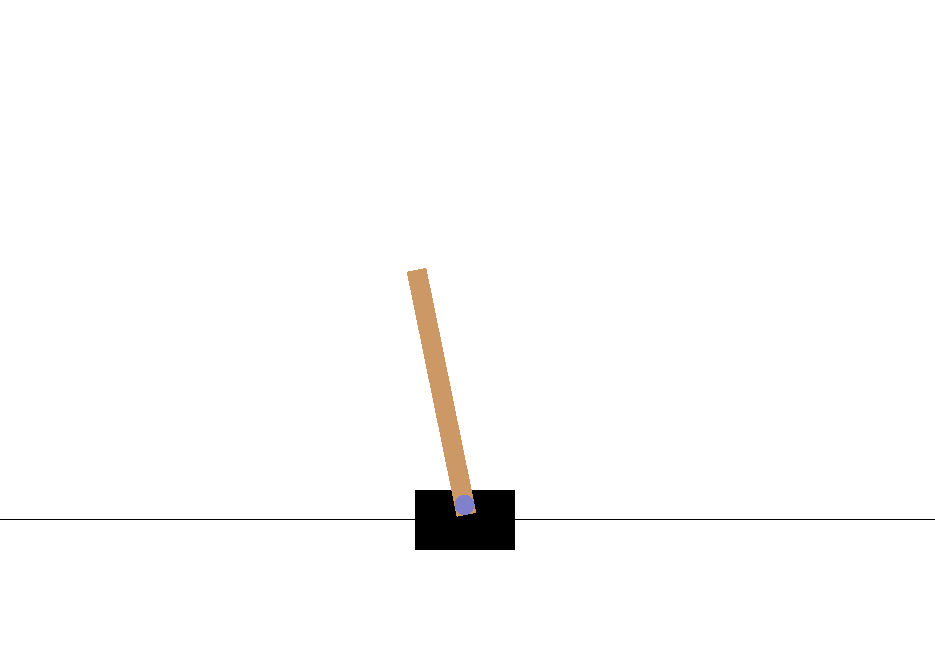
\includegraphics[width=8cm]{policy_gradient/env.png}
\end{center}

We have included a simple simulator for this problem. The simulation proceeds in discrete time cycles (steps). The state of the cart and pole at any time is completely characterized by 4 scalar values: the cart position, the cart velocity, the angle of the pole measured as its deviation from the vertical position, and the angular velocity of the pole. The concatenation of these 4 scalar values is the state $s$. 

\newcommand{\tilT}{\tilde{T}}
At every time step, the controller must choose one of two actions: push (accelerate) the cart left, or push the cart right. (To keep the problem simple, there is no {\it do-nothing} action.) \textbf{These are represented as actions $0$ and $1$ respectively in the code.}  When the action choice is made, the simulator updates the state according to the underlying dynamics, and provides a new state. 
If the angle of the pole deviates by more than a certain amount from the vertical position, or if the cart's position goes out of bounds, we conceptually consider that the MDP enters a special ``done'' state, and once the MDP enters the ``done'' state, no actions can recover it to any normal state. 
We choose the horizon $T$ to be 200, meaning, we only take at most 200 actions in each trajectory. Note because once the system enters the ``done'' state, it stays there forever, we do not have to simulate the MDP and sample more states anymore after the first time we enter the done state (and all future done states can be ignored because no actions can influence anything). Therefore, in the code, you will only interact with the simulation until the system hits the done state (or reaches a trajectory length of 200), so the effective length of the trajectory can be less than 200. We use $\tilT$ to denote the number of steps with which a trajectory reaches a ``done'' state or 200 otherwise. The discount factor will be set to $\gamma=1$ throughout the question. 


Our goal is to make the pole and cart stay in bounds without entering the done state for as many steps as possible. To do this, we design the following reward function.  For any normal state $s\in \R^4$, we have $R(s)=1$ (and $R$ does not depend on the action $a$). When the system is at the ``done" state (that is, the pole angle goes beyond a certain limit or when the cart goes too far out), the reward is 0. The reward is given to you in the code as part of the MDP. 

The files for this problem are contained within the \texttt{src/policy\_gradient/} directory. Most of the scaffolding code has already been written for you, and you need to make changes only to {\tt policy\_gradient.py} in the places specified. There are also several details that are also clearly outlined inside of the code. This file can then be run to display the behavior of the agent in real time, and to plot a learning curve of the agent at the end.

\begin{enumerate}
\item \subquestionpoints{6} 
\textbf{Policy Gradient}

In this part, we will fully detail the characterization of our policy gradient method and derive the update rule to train our model to solve the {\tt CartPole-v0} environment.

In this problem we will be learning a \textit{logistic} policy. This means that our policy will be a sigmoid function of a linear function in the state. 
Recall that the sigmoid function $\sigma(z) = 1 / (1 + e^{-z})$. Let $\theta \in \R^4$ be the parameters of the policy. 
The probability of taking action 0 (left) is parameterized by 
\begin{align*}
    \pi_\theta(0 | s) &= \sigma(\theta^\top s) 
\end{align*}
Given that our environment only contains two actions, the probability of taking action 1 (right) is simply one minus the probability of taking action 0 (left). To be concrete:
\begin{align*}
\pi_\theta(1 | s) &= 1 - \pi_\theta(0 | s) = \sigma(-\theta^\top s)
\end{align*}

Now recall the gradient of our objective $\eta(\theta)$ in the context of vanilla policy gradient, which is given by the following expression. This value acts as an estimator for the gradient of the expected cumulative reward with respect to the policy parameters.

\begin{align*}
    \nabla_\theta \eta(\theta) = \sum_{t=0}^{\tilT - 1} \E_{\tau \sim P_\theta} \left[ \nabla_\theta \ln \pi_\theta(a_t | s_t) \cdot \left( \sum_{j = 0}^{\tilT - 1}R(s_j, a_j) \right) \right]
\end{align*}

Note that this is slightly different from the formula given in the lecture notes because a) the discount factor $\gamma=1$ in this question, and b) we dropped everything after time step $\tilT$ because once the trajectory enters the done state, all the rewards become zero and the parameter $\theta$ doesn't influence $\eta(\theta)$ anymore. 

Before we are able to implement our algorithm, we will need to first derive the expression for $\nabla_\theta \ln \pi_\theta(a | s)$. 
\textbf{Derive this value for each action, namely $\nabla_\theta \ln \pi_\theta(0 | s)$ and $\nabla_\theta \ln \pi_\theta(1 | s)$.} Both of your answers should be as simplified as possible and in terms of $\theta$, $s$, and the sigmoid function $\sigma(\cdot)$.


\ifnum\solutions=1 {
  \begin{answer}
\end{answer}

} \fi

\item \subquestionpoints{22} 
\textbf{Implementation}

Now that we've derived the gradient which will be used to update our model parameters, follow the instructions in {\tt src/policy\_gradient/policy\_gradient.py} to implement the algorithm. \textbf{In particular, implement the following functions:}

\begin{enumerate}
    \item \texttt{sigmoid(x)}
    \item \texttt{policy(state)}
    \item \texttt{sample\_action(state)}
    \item \texttt{grad\_log\_prob(state)}
    \item \texttt{compute\_weights\_full\_trajectory(episode\_rewards)}
    \item \texttt{update(episode\_rewards, states, actions)}
\end{enumerate}

Once you've finished implementing the above functions, run the experiment via {\tt python policy\_gradient.py}. Include the generated plot \texttt{full\_trajectory.png} in your write-up.

\ifnum\solutions=1 {
  \begin{answer}
\end{answer}

} \fi

\item \subquestionpoints{7} 
\textbf{Reward-To-Go}

An approach to reducing the variance of the policy gradient is to exploit the fact that our policy cannot impact rewards in the past. This yields the following modified gradient estimator, referred to as the \textit{reward-to-go}, where we multiply $\nabla_\theta \ln \pi(a_t | s_t)$ at each individual time step $t$ by the the sum of future rewards from that time step onward (instead of for all time steps as we did before). The gradient of the objective is given by the following expression:

\begin{align*}
    \nabla_\theta \eta(\theta) = \sum_{t=0}^{\tilT-1} \E_{\tau \sim P_\theta} \left[ \nabla_\theta \ln \pi(a_t | s_t) \cdot \left( \sum_{j \geq t}^{\tilT - 1} R(s_j, a_j) \right) \right]
\end{align*}


Follow the instructions in \texttt{src/policy\_gradient/policy\_gradient.py} to \textbf{implement the function \texttt{compute\_weights\_reward\_to\_go(episode\_rewards)}}. Once you're done, run the new experiment via {\tt python policy\_gradient.py --weighting reward\_to\_go }. \textbf{Include the generated plot {\tt reward\_to\_go.png } in your write-up}. Now, \textbf{briefly compare the two plots qualitatively} - how does this plot compare to the previous one? Does one estimator of the gradient seem preferable over the other, and what qualities make you say this?


\ifnum\solutions=1 {
  \begin{answer}
\end{answer}

} \fi
\end{enumerate}


\clearpage
\item \points{35} {\bf Reinforcement Learning: Policy Gradient}

Before working on this problem, please run \texttt{pip install gym==0.17.3} to install the OpenAI Gym Python dependency.

In this problem you will investigate reinforcement learning, in particular policy gradient methods, as an approach to solving control tasks without explicit knowledge of the dynamics of the underlying system.

The problem we will consider is the inverted pendulum problem, also referred to as the pole-balancing problem, provided in the form of the {\tt CartPole-v0} OpenAI Gym environment.\footnote{{\tt https://gym.openai.com/envs/CartPole-v0/}} 
The physics setup and details of the MDP are described below, although you do not necessarily have to understand all the details to solve the problem. 
As shown in the figure below, a thin pole is connected via a free hinge to a cart, which can move laterally on a smooth table surface. 
Our objective is to develop a controller/policy to balance the pole with these  constraints by appropriately having the cart accelerate either left or right. The controller/policy is considered as failed if either the angle of the pole deviates by more than a certain amount from the vertical position (i.e., if the pole falls over), or if the cart's position goes out of bounds (i.e., if it falls off the end of the table by going too far left or right). 

\begin{center}
  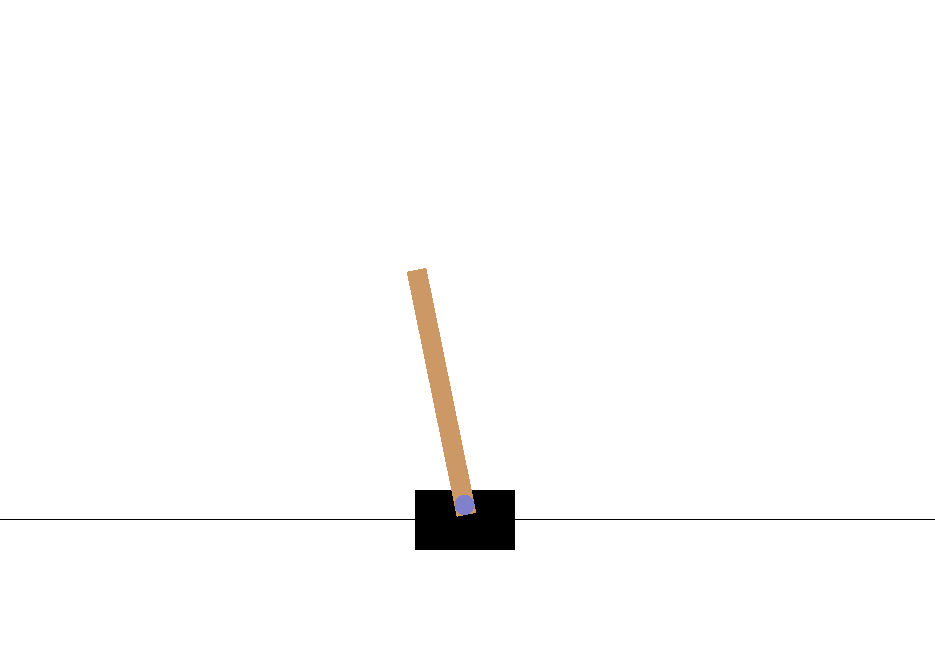
\includegraphics[width=8cm]{policy_gradient/env.png}
\end{center}

We have included a simple simulator for this problem. The simulation proceeds in discrete time cycles (steps). The state of the cart and pole at any time is completely characterized by 4 scalar values: the cart position, the cart velocity, the angle of the pole measured as its deviation from the vertical position, and the angular velocity of the pole. The concatenation of these 4 scalar values is the state $s$. 

\newcommand{\tilT}{\tilde{T}}
At every time step, the controller must choose one of two actions: push (accelerate) the cart left, or push the cart right. (To keep the problem simple, there is no {\it do-nothing} action.) \textbf{These are represented as actions $0$ and $1$ respectively in the code.}  When the action choice is made, the simulator updates the state according to the underlying dynamics, and provides a new state. 
If the angle of the pole deviates by more than a certain amount from the vertical position, or if the cart's position goes out of bounds, we conceptually consider that the MDP enters a special ``done'' state, and once the MDP enters the ``done'' state, no actions can recover it to any normal state. 
We choose the horizon $T$ to be 200, meaning, we only take at most 200 actions in each trajectory. Note because once the system enters the ``done'' state, it stays there forever, we do not have to simulate the MDP and sample more states anymore after the first time we enter the done state (and all future done states can be ignored because no actions can influence anything). Therefore, in the code, you will only interact with the simulation until the system hits the done state (or reaches a trajectory length of 200), so the effective length of the trajectory can be less than 200. We use $\tilT$ to denote the number of steps with which a trajectory reaches a ``done'' state or 200 otherwise. The discount factor will be set to $\gamma=1$ throughout the question. 


Our goal is to make the pole and cart stay in bounds without entering the done state for as many steps as possible. To do this, we design the following reward function.  For any normal state $s\in \R^4$, we have $R(s)=1$ (and $R$ does not depend on the action $a$). When the system is at the ``done" state (that is, the pole angle goes beyond a certain limit or when the cart goes too far out), the reward is 0. The reward is given to you in the code as part of the MDP. 

The files for this problem are contained within the \texttt{src/policy\_gradient/} directory. Most of the scaffolding code has already been written for you, and you need to make changes only to {\tt policy\_gradient.py} in the places specified. There are also several details that are also clearly outlined inside of the code. This file can then be run to display the behavior of the agent in real time, and to plot a learning curve of the agent at the end.

\begin{enumerate}
\item \subquestionpoints{6} 
\textbf{Policy Gradient}

In this part, we will fully detail the characterization of our policy gradient method and derive the update rule to train our model to solve the {\tt CartPole-v0} environment.

In this problem we will be learning a \textit{logistic} policy. This means that our policy will be a sigmoid function of a linear function in the state. 
Recall that the sigmoid function $\sigma(z) = 1 / (1 + e^{-z})$. Let $\theta \in \R^4$ be the parameters of the policy. 
The probability of taking action 0 (left) is parameterized by 
\begin{align*}
    \pi_\theta(0 | s) &= \sigma(\theta^\top s) 
\end{align*}
Given that our environment only contains two actions, the probability of taking action 1 (right) is simply one minus the probability of taking action 0 (left). To be concrete:
\begin{align*}
\pi_\theta(1 | s) &= 1 - \pi_\theta(0 | s) = \sigma(-\theta^\top s)
\end{align*}

Now recall the gradient of our objective $\eta(\theta)$ in the context of vanilla policy gradient, which is given by the following expression. This value acts as an estimator for the gradient of the expected cumulative reward with respect to the policy parameters.

\begin{align*}
    \nabla_\theta \eta(\theta) = \sum_{t=0}^{\tilT - 1} \E_{\tau \sim P_\theta} \left[ \nabla_\theta \ln \pi_\theta(a_t | s_t) \cdot \left( \sum_{j = 0}^{\tilT - 1}R(s_j, a_j) \right) \right]
\end{align*}

Note that this is slightly different from the formula given in the lecture notes because a) the discount factor $\gamma=1$ in this question, and b) we dropped everything after time step $\tilT$ because once the trajectory enters the done state, all the rewards become zero and the parameter $\theta$ doesn't influence $\eta(\theta)$ anymore. 

Before we are able to implement our algorithm, we will need to first derive the expression for $\nabla_\theta \ln \pi_\theta(a | s)$. 
\textbf{Derive this value for each action, namely $\nabla_\theta \ln \pi_\theta(0 | s)$ and $\nabla_\theta \ln \pi_\theta(1 | s)$.} Both of your answers should be as simplified as possible and in terms of $\theta$, $s$, and the sigmoid function $\sigma(\cdot)$.


\ifnum\solutions=1 {
  \begin{answer}
\end{answer}

} \fi

\item \subquestionpoints{22} 
\textbf{Implementation}

Now that we've derived the gradient which will be used to update our model parameters, follow the instructions in {\tt src/policy\_gradient/policy\_gradient.py} to implement the algorithm. \textbf{In particular, implement the following functions:}

\begin{enumerate}
    \item \texttt{sigmoid(x)}
    \item \texttt{policy(state)}
    \item \texttt{sample\_action(state)}
    \item \texttt{grad\_log\_prob(state)}
    \item \texttt{compute\_weights\_full\_trajectory(episode\_rewards)}
    \item \texttt{update(episode\_rewards, states, actions)}
\end{enumerate}

Once you've finished implementing the above functions, run the experiment via {\tt python policy\_gradient.py}. Include the generated plot \texttt{full\_trajectory.png} in your write-up.

\ifnum\solutions=1 {
  \begin{answer}
\end{answer}

} \fi

\item \subquestionpoints{7} 
\textbf{Reward-To-Go}

An approach to reducing the variance of the policy gradient is to exploit the fact that our policy cannot impact rewards in the past. This yields the following modified gradient estimator, referred to as the \textit{reward-to-go}, where we multiply $\nabla_\theta \ln \pi(a_t | s_t)$ at each individual time step $t$ by the the sum of future rewards from that time step onward (instead of for all time steps as we did before). The gradient of the objective is given by the following expression:

\begin{align*}
    \nabla_\theta \eta(\theta) = \sum_{t=0}^{\tilT-1} \E_{\tau \sim P_\theta} \left[ \nabla_\theta \ln \pi(a_t | s_t) \cdot \left( \sum_{j \geq t}^{\tilT - 1} R(s_j, a_j) \right) \right]
\end{align*}


Follow the instructions in \texttt{src/policy\_gradient/policy\_gradient.py} to \textbf{implement the function \texttt{compute\_weights\_reward\_to\_go(episode\_rewards)}}. Once you're done, run the new experiment via {\tt python policy\_gradient.py --weighting reward\_to\_go }. \textbf{Include the generated plot {\tt reward\_to\_go.png } in your write-up}. Now, \textbf{briefly compare the two plots qualitatively} - how does this plot compare to the previous one? Does one estimator of the gradient seem preferable over the other, and what qualities make you say this?


\ifnum\solutions=1 {
  \begin{answer}
\end{answer}

} \fi
\end{enumerate}


\clearpage
\item \points{35} {\bf Reinforcement Learning: Policy Gradient}

Before working on this problem, please run \texttt{pip install gym==0.17.3} to install the OpenAI Gym Python dependency.

In this problem you will investigate reinforcement learning, in particular policy gradient methods, as an approach to solving control tasks without explicit knowledge of the dynamics of the underlying system.

The problem we will consider is the inverted pendulum problem, also referred to as the pole-balancing problem, provided in the form of the {\tt CartPole-v0} OpenAI Gym environment.\footnote{{\tt https://gym.openai.com/envs/CartPole-v0/}} 
The physics setup and details of the MDP are described below, although you do not necessarily have to understand all the details to solve the problem. 
As shown in the figure below, a thin pole is connected via a free hinge to a cart, which can move laterally on a smooth table surface. 
Our objective is to develop a controller/policy to balance the pole with these  constraints by appropriately having the cart accelerate either left or right. The controller/policy is considered as failed if either the angle of the pole deviates by more than a certain amount from the vertical position (i.e., if the pole falls over), or if the cart's position goes out of bounds (i.e., if it falls off the end of the table by going too far left or right). 

\begin{center}
  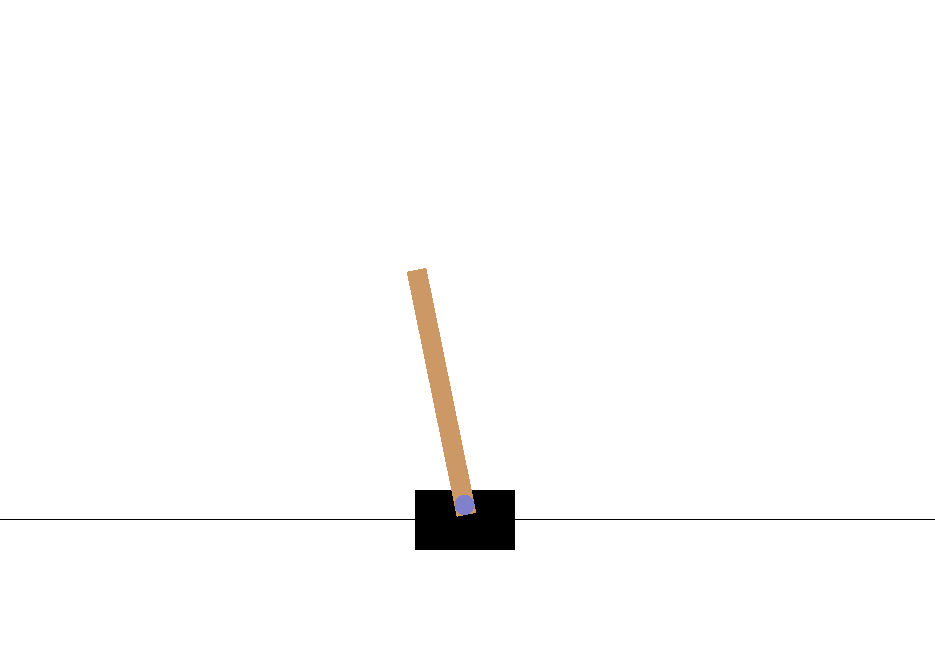
\includegraphics[width=8cm]{policy_gradient/env.png}
\end{center}

We have included a simple simulator for this problem. The simulation proceeds in discrete time cycles (steps). The state of the cart and pole at any time is completely characterized by 4 scalar values: the cart position, the cart velocity, the angle of the pole measured as its deviation from the vertical position, and the angular velocity of the pole. The concatenation of these 4 scalar values is the state $s$. 

\newcommand{\tilT}{\tilde{T}}
At every time step, the controller must choose one of two actions: push (accelerate) the cart left, or push the cart right. (To keep the problem simple, there is no {\it do-nothing} action.) \textbf{These are represented as actions $0$ and $1$ respectively in the code.}  When the action choice is made, the simulator updates the state according to the underlying dynamics, and provides a new state. 
If the angle of the pole deviates by more than a certain amount from the vertical position, or if the cart's position goes out of bounds, we conceptually consider that the MDP enters a special ``done'' state, and once the MDP enters the ``done'' state, no actions can recover it to any normal state. 
We choose the horizon $T$ to be 200, meaning, we only take at most 200 actions in each trajectory. Note because once the system enters the ``done'' state, it stays there forever, we do not have to simulate the MDP and sample more states anymore after the first time we enter the done state (and all future done states can be ignored because no actions can influence anything). Therefore, in the code, you will only interact with the simulation until the system hits the done state (or reaches a trajectory length of 200), so the effective length of the trajectory can be less than 200. We use $\tilT$ to denote the number of steps with which a trajectory reaches a ``done'' state or 200 otherwise. The discount factor will be set to $\gamma=1$ throughout the question. 


Our goal is to make the pole and cart stay in bounds without entering the done state for as many steps as possible. To do this, we design the following reward function.  For any normal state $s\in \R^4$, we have $R(s)=1$ (and $R$ does not depend on the action $a$). When the system is at the ``done" state (that is, the pole angle goes beyond a certain limit or when the cart goes too far out), the reward is 0. The reward is given to you in the code as part of the MDP. 

The files for this problem are contained within the \texttt{src/policy\_gradient/} directory. Most of the scaffolding code has already been written for you, and you need to make changes only to {\tt policy\_gradient.py} in the places specified. There are also several details that are also clearly outlined inside of the code. This file can then be run to display the behavior of the agent in real time, and to plot a learning curve of the agent at the end.

\begin{enumerate}
\item \subquestionpoints{6} 
\textbf{Policy Gradient}

In this part, we will fully detail the characterization of our policy gradient method and derive the update rule to train our model to solve the {\tt CartPole-v0} environment.

In this problem we will be learning a \textit{logistic} policy. This means that our policy will be a sigmoid function of a linear function in the state. 
Recall that the sigmoid function $\sigma(z) = 1 / (1 + e^{-z})$. Let $\theta \in \R^4$ be the parameters of the policy. 
The probability of taking action 0 (left) is parameterized by 
\begin{align*}
    \pi_\theta(0 | s) &= \sigma(\theta^\top s) 
\end{align*}
Given that our environment only contains two actions, the probability of taking action 1 (right) is simply one minus the probability of taking action 0 (left). To be concrete:
\begin{align*}
\pi_\theta(1 | s) &= 1 - \pi_\theta(0 | s) = \sigma(-\theta^\top s)
\end{align*}

Now recall the gradient of our objective $\eta(\theta)$ in the context of vanilla policy gradient, which is given by the following expression. This value acts as an estimator for the gradient of the expected cumulative reward with respect to the policy parameters.

\begin{align*}
    \nabla_\theta \eta(\theta) = \sum_{t=0}^{\tilT - 1} \E_{\tau \sim P_\theta} \left[ \nabla_\theta \ln \pi_\theta(a_t | s_t) \cdot \left( \sum_{j = 0}^{\tilT - 1}R(s_j, a_j) \right) \right]
\end{align*}

Note that this is slightly different from the formula given in the lecture notes because a) the discount factor $\gamma=1$ in this question, and b) we dropped everything after time step $\tilT$ because once the trajectory enters the done state, all the rewards become zero and the parameter $\theta$ doesn't influence $\eta(\theta)$ anymore. 

Before we are able to implement our algorithm, we will need to first derive the expression for $\nabla_\theta \ln \pi_\theta(a | s)$. 
\textbf{Derive this value for each action, namely $\nabla_\theta \ln \pi_\theta(0 | s)$ and $\nabla_\theta \ln \pi_\theta(1 | s)$.} Both of your answers should be as simplified as possible and in terms of $\theta$, $s$, and the sigmoid function $\sigma(\cdot)$.


\ifnum\solutions=1 {
  \begin{answer}
\end{answer}

} \fi

\item \subquestionpoints{22} 
\textbf{Implementation}

Now that we've derived the gradient which will be used to update our model parameters, follow the instructions in {\tt src/policy\_gradient/policy\_gradient.py} to implement the algorithm. \textbf{In particular, implement the following functions:}

\begin{enumerate}
    \item \texttt{sigmoid(x)}
    \item \texttt{policy(state)}
    \item \texttt{sample\_action(state)}
    \item \texttt{grad\_log\_prob(state)}
    \item \texttt{compute\_weights\_full\_trajectory(episode\_rewards)}
    \item \texttt{update(episode\_rewards, states, actions)}
\end{enumerate}

Once you've finished implementing the above functions, run the experiment via {\tt python policy\_gradient.py}. Include the generated plot \texttt{full\_trajectory.png} in your write-up.

\ifnum\solutions=1 {
  \begin{answer}
\end{answer}

} \fi

\item \subquestionpoints{7} 
\textbf{Reward-To-Go}

An approach to reducing the variance of the policy gradient is to exploit the fact that our policy cannot impact rewards in the past. This yields the following modified gradient estimator, referred to as the \textit{reward-to-go}, where we multiply $\nabla_\theta \ln \pi(a_t | s_t)$ at each individual time step $t$ by the the sum of future rewards from that time step onward (instead of for all time steps as we did before). The gradient of the objective is given by the following expression:

\begin{align*}
    \nabla_\theta \eta(\theta) = \sum_{t=0}^{\tilT-1} \E_{\tau \sim P_\theta} \left[ \nabla_\theta \ln \pi(a_t | s_t) \cdot \left( \sum_{j \geq t}^{\tilT - 1} R(s_j, a_j) \right) \right]
\end{align*}


Follow the instructions in \texttt{src/policy\_gradient/policy\_gradient.py} to \textbf{implement the function \texttt{compute\_weights\_reward\_to\_go(episode\_rewards)}}. Once you're done, run the new experiment via {\tt python policy\_gradient.py --weighting reward\_to\_go }. \textbf{Include the generated plot {\tt reward\_to\_go.png } in your write-up}. Now, \textbf{briefly compare the two plots qualitatively} - how does this plot compare to the previous one? Does one estimator of the gradient seem preferable over the other, and what qualities make you say this?


\ifnum\solutions=1 {
  \begin{answer}
\end{answer}

} \fi
\end{enumerate}


\end{enumerate}

\end{document}
